\subsection{Variations}
\label{ssec:relating-variations}

We now discuss some variations on the case of binary heterogeneous
synchronisations in the previous section.  We give a general construction in
the next section, but we consider the constructions in this section to be
easier to understand: to a certain extent, this section can be seen as
providing stepping stones towards that general construction. 

The results of the previous subsections carry across to non-binary, fixed
arity synchronisations, in a straightforward way.  For a $k$-way
synchronisation between distinct operations |op|\s1, \ldots, |op|$_k$, the
corresponding two-step linearisation specification object has $2k-1$
operations, |op|\s1, \ldots, |op|$_k$, $\overline{\sm{op}}_1$, \ldots,
$\overline{\sm{op}}_{k-1}$.  The definition of two-step linearisation is then
the obvious adaptation of the binary case: each operation |op|\s{i} of the
synchronisation object is linearised by the composition of |op|\s{i} and
$\overline{\op}_i$ of the specification object, for $i = 1, \ldots, k-1$.

The construction of the previous subsection is easily adapted to the case of
$k$-way synchronisations for $k > 2$.  The specification object encodes an
automaton with $k$ states.  The figure below gives the automaton in the case
$k = 4$.
%
\begin{center}
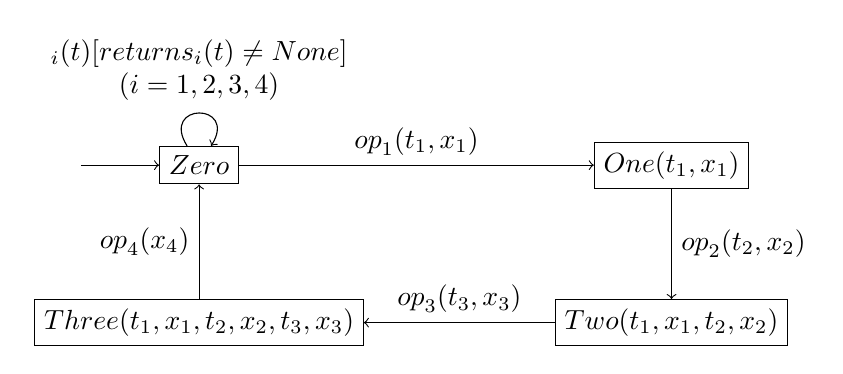
\begin{tikzpicture}[xscale = 1]
\draw (0,0) node[draw] (zero) {$\sm{Zero}$};
\draw[->] (zero) ++ (-1.5, 0) -- (zero);
\draw[->] (zero) .. controls ++(-0.5,+0.8) and ++(0.5,0.8) .. 
  node[above]{
    $\begin{array}{c}
      \overline{\op}_i(t) [\sm{returns}_i(t) \ne \sm{None}] \\ (i = 1,2,3,4)
    \end{array}$}
  (zero);
%
\draw (zero)++(6,0) node[draw] (one) {$\sm{One}(\sm{t}_1, \sm{x}_1)$};
\draw[->] (zero)  -- node[above] {$\sm{op}_1(\sm{t}_1, \sm{x}_1)$} (one); 
%
\draw (one)++(0, -2) node[draw] (two) 
  {$\sm{Two}(\sm{t}_1, \sm{x}_1, \sm{t}_2, \sm{x}_2)$};
\draw[->] (one)  -- node[right] {$\sm{op}_2(\sm{t}_2, \sm{x}_2)$} (two); 
%
\draw (two)++(-6, 0) node[draw] (three) 
  {$\sm{Three}(\sm{t}_1, \sm{x}_1, \sm{t}_2, \sm{x}_2, \sm{t}_3, \sm{x}_3)$};
\draw[->] (two)  -- node[above] {$\sm{op}_3(\sm{t}_3, \sm{x}_3)$} (three); 
%
\draw[->] (three)  -- node[left] {$\sm{op}_4(\sm{x}_4)$} (zero);
\end{tikzpicture}
\end{center}
%
The final |op| operation, |op|\s4 in the above figure, applies the |sync|
method of the synchronisation specification object to the parameters $\sm x_1,
\ldots, \sm x_k$ to obtain the results $\sm y_1, \ldots, \sm y_k$; it stores
the first $k-1$ in appropriate |returns|\s{i} arrays, and returns $\sm y_k$
itself.  In the case $k=4$, it has definition:
%
\begin{scala}
  def op£\s4£(x£\s4£: A£\s4£): B£\s4£ = {
    require(state.isInstanceOf[Three]); val Three(t£\s1£, x£\s1£, t£\s2£, x£\s2£, t£\s3£, x£\s3£) = state
    val (y£\s1£, y£\s2£, y£\s3£, y£\s4£) = SyncSpec.sync(x£\s1£, x£\s2£, x£\s3£, x£\s4£) 
    returns£\s1£(t£\s1£) = Some(y£\s1£); returns£\s2£(t£\s2£) = Some(y£\s2£); returns£\s3£(t£\s3£) = Some(y£\s3£)
    state = Zero; y£\s4£
  }
\end{scala}
%
Each $\overline{\sm{op}}_i$ operation retrieves the result from the
corresponding |returns|\s{i} array.

%%%%%%%%%%%%%%%%%%%%%%%%%%%%%%%%%%%%%%%%%%%%%%%%%% Homogeneous

\begin{window}[0,r,{%
\begin{minipage}{39mm}
\begin{tikzpicture}[>= angle 60, xscale = 0.9, yscale = 0.44]
\draw (0,0) node[draw] (zero) {$\sm{Zero}$};
\draw[->] (zero) ++ (-1.5, 0) -- (zero);
\loopAbove(zero){$\begin{array}{c}
  \overline\op(\sm t) \\ {[\sm{returns(t)} \ne \sm{None}]}
  \end{array}$}
%
\draw (0,-4) node[draw] (one) {$\sm{One}(\sm t_1, \sm{x}_1)$};
\draw[->] (zero) .. controls ++(0.3,-2) .. 
  node[right] {$\sm{op}(\sm t_1, \sm{x}_1)$} (one); 
%
\draw[->] (one) .. controls ++(-0.3,2) .. 
  node[left] {$\sm{op}(\sm t_2, \sm x_2)$} (zero);
\end{tikzpicture}%
\end{minipage}
},]
We now consider the homogeneous case.  For simplicity, we describe the binary
case; synchronisations of more than two operation executions are handled
similarly.  Suppose we have a synchronisation object with a single operation
%\protect\SCALA{def op(x: A): B}.  
{\bfseries\scalastyle def}~{\scalastyle op(x: A): B}.  
All executions of~|op| have to be treated similarly,
so we associate \emph{each} with two operations |op| and $\overline{\sm{op}}$
of the specification object.  The specification object is below, and encodes
the automaton on the right.
The second execution of |op| in any synchronisation (from the |One| state of the
automaton) writes the results of the execution into the |returns| array.
Each execution of $\overline{\sm{op}}$ returns the stored value.
\end{window}
%
%% \begin{trivlist}
%% \item[]
%\begin{minipage}{92mm}
\begin{scala}
class TwoStepHomoLinSpec{
  private var state: State = Zero
  private val returns = new Array[Option[B£\s1£]](NumThreads)
  for(t <- 0 until NumThreads) returns(t) = None
  def op(t: ThreadID, x: A): Unit = {
    require(returns(t) == None)
    state match{
      case Zero => state = One(t, x)
      case One(t£\s1£, x£\s1£) => 
        val (y£\s1£, y£\s2£) = SyncSpec.sync(x£\s1£, x) 
        returns(t£\s1£) = Some(y£\s1£); returns(t) = Some(y£\s2£); state = Zero
    }
  }
  def £$\overline{\sm{op}}$£(t: ThreadID): B = {
    require(state.isInstanceOf[Zero] && returns(t).isInstanceOf[Some])
    val Some(y) = returns(t); returns(t) = None; y
  }
}
\end{scala}


%%%%%%%%%%%%%%%%%%%%%%%%%%%%%%%%%%%%%%%%%%%%%%%%%%%%%%% Mixed arity

Recall that some operations have multiple modes of synchronisations: different
executions of the operation may have synchronisations with different arities.
For example, in a timeout channel, an execution of the |send| and |receive|
operations may synchronise with an execution of the other operation, or may
timeout corresponding to a unary synchronisation.

\begin{window}[0,r,{
\begin{minipage}{52.9mm}
\begin{tikzpicture}[>= angle 60, xscale = 0.9, yscale = 0.44]
\draw (0,0) node[draw] (zero) {$\sm{Zero}$};
\draw[->] (zero) ++ (-1.5, 0) -- (zero);
% self-loop on Zero
\loopAbove(zero){$\begin{array}{@{}c@{}}
      \receive()\::\sm{None}, \\ 
      \overline{\send}(\sm t)\::\sm{true} [\sm{returns(t)} \ne \sm{None}]
    \end{array}$}
%%%%%% One
\draw (0,-5) node[draw] (one) {$\sm{One}(\sm t, \sm{x})$};
\draw[->] (zero) .. controls ++(0.3,-2.5) .. 
  node[right] {$\send(\sm t, \sm{x})$} (one); 
\draw[->] (one) .. controls ++(-0.3,2.5) .. 
  node[left] {$\begin{array}[t]{@{}r@{}}
   \receive()\::\sm{Some(x)}, \\ \overline{\send}(\sm t)\::\sm{false}
    \end{array}$} (zero);
\end{tikzpicture}
\end{minipage}
},] 
The figure to the right gives the automaton for a timeout
channel, where we treat $\send$ as corresponding to $\op_1$ (we omit concrete
code in the interests of brevity).  The automaton is similar to that for a
standard channel.  The |receive| operation can happen from either state: if it
happens from the |One| state, then a synchronisation has occurred and the
execution returns a value of the form |Some(x)|; but if it happens from the
|Zero| state, there has been no corresponding |send|, and so the execution
returns~|None|, indicating a timeout.  Likewise, the $\overline{\send}$
operation can happen from either state; if it happens from the |Zero| state,
then a synchronisation has occurred and the execution returns |true|; but if
it happens from the |One| state, there has been no corresponding |receive|,
and so the execution returns~|false|, indicating a timeout.
\end{window}



%%%%%%%%%%%%%%%%%%%%%%%%%%%%%%%%%%%%%%%%%%%%%%%%%%%%%%% Stateful

We now consider stateful specification objects.  In general, we can simply
augment the |Zero| and |One| states of the automaton to include the state of
the specification object.  Different transitions may be available
based upon that state.  However, it can be clearer and simpler to introduce
different named states into the automaton.

The figure below gives the specification automaton for a closeable channel.
%
%\begin{figure}
\begin{center}
\begin{tikzpicture}[>= angle 60, xscale = 0.9, yscale = 0.44]
\draw (0,0) node[draw] (zero) {$\sm{Zero}$};
\draw[->] (zero) ++ (-1.5, 0) -- (zero);
% self-loop on Zero
\loopAbove(zero){$\begin{array}{@{}c@{}}
  \overline{\send}(\sm t) \\ {[\sm{returns(t)} \ne \sm{None}]}
  \end{array}$}
%%%%%% One
\draw (0,-5) node[draw] (one) {$\sm{One}(\sm t, \sm{x})$};
\draw[->] (zero) .. controls ++(0.3,-2.5) .. 
  node[right] {$\send(\sm t, \sm{x})$} (one); 
\draw[->] (one) .. controls ++(-0.3,2.5) .. 
  node[left] {$\receive()$} (zero);
%%%%%% Closed
\draw (4.5,0) node[draw] (closed) {$\sm{Closed}$};
\draw[->] (zero) -- node[above] {$\sm{close}$} (closed);
% self-loop on closed
\loopAbove(closed){$\begin{array}{@{}c@{}}
      %% \overline{\send}(\sm t) [\sm{returns(t)} \ne \sm{None}], \\
      %% \send(\sm t), \, \receive(), \, \sm{close} 
      \overline{\send}(\sm t), \send(\sm t, \sm x), \\ \receive(), \, \sm{close}() 
    \end{array}$} 
\end{tikzpicture}
\end{center}
%% \caption{Automaton for capturing two-step linearisation for a closeable
%%   channel.}
%% \label{fig:two-step-closeable-chan}
%% \end{figure}
%
The automaton has an additional state, |Closed|,
corresponding to the channel being closed.  All executions are unary
synchronisations in this state.  This automaton represents a simplification
over the general approach discussed above: we do not need two separate states
after closing.  Note that a $\overline{\send}(\sm t)$ transition from the
|Closed| state may succeed if the corresponding synchronisation happened
before the channel was closed, in which case $\sm{returns(t)} \ne \sm{None}$.

%%%%%%%%%%

\subsection{The general construction}
\label{ssec:relating-general}

We now give a general construction to show how two-step linearisation can
capture synchronisation linearisation. 
%
Fix a synchronisation object~|SyncObj|, a synchronisation specification object
|SyncSpec|, and synchronisation abstraction function~$\A$.  Let the operations
of the |SyncObj| be
\begin{scala}
  def op£\s i£(x: A£\s i£): B£\s i \qquad for $i = 1,\ldots,n$.£
\end{scala}

The two-step linearisation tester has operations $\op_i$ and
$\overline\op_i$ for $i = 1,\ldots,n$. 
%
The idea is that for a mapping 
\[
\seq{\op_{i_i}(x_1), \ldots, \op_{i_a}(x_a)}
  \mapsto \sync(x_1,\ldots,x_a)  \in \A,
\]
corresponding to a synchronisation of arity~$a$, is linearised in the
following order:
\begin{enumerate}
\item $\op_{i_1},\ldots,\op_{i_a}$, in order;

\item $\overline\op_{i_i}$, for some~$i$, which  calls
  |SyncSpec.sync|$(x_1,\ldots,x_a)$, and stores the results for other threads;

\item The remaining $\overline\op_{i_j}$, in some order, which  retrieve
  their results.
\end{enumerate}
%
No other operation occurs between the start of stage~1 until after
stage~2; but other operations may occur during stage~3.

During stage~1, the two-step linearisabilty tester  records the prefix of
$\seq{\op_{i_i}(x_1), \ldots, \op_{i_a}(x_a)}$ performed so far.  This is done
by defining a case class |Op|$_i$ corresponding to each such
operation~|op|$_i$, as at the top of Figure~\ref{fig:schema}.
%
%% \begin{scala}
%% trait Op
%% case class Op_i(t: ThreadID, x: A_i) £\quad for $i = 1,...,n$.£
%% type State = List[Op]
%% \end{scala}
%
The following function maps such a sequence to the corresponding sequence of
operations, for use with~$\A$.
\begin{eqnarray*}
\opsFor(state) &  = & \seq{\op_j(x_j) \midd \sm{Op}_j(t_j,x_j) \leftarrow state}.
\end{eqnarray*}

A schema (using pseudo-Scala) for the general construction is in
Figure~\ref{fig:schema}.  The variable~|state| records the sequence of
|op|$_i$ linearised so far: this satisfies an invariant that it is a prefix of
an element of $\dom \A$.  For each thread~|t|,\, |returns(t)| stores the value
to be returned by~|t| as part of its most recent uncompleted synchronisation,
if any. % , where $B = \bigcup\nolimits_{i = 1,\ldots,n} \sm B_i$.

%%%%%

\begin{figure}
\begin{scala}
trait Op
case class Op£$_i$£(t: ThreadID, x: A£$_i$£) //  for £$i = 1,...,n$.£
type State = List[Op]
type B = £$\bigcup\nolimits_{i = 1,\ldots,n} \sm B_i$£

class TwoStepLinSpec{
  private var state: State = List()
  private val returns = Array.fill[Option[B]](NumThreads)(None) 

  def op£\s i£(t: ThreadID, x: A£\s i£): Unit = { // for £$i = 1,...,n$£.
    require(£$\exists ops \in \dom \A \spot \opsFor(\sm{state}) \cat \seq{\op_i(x)} \prefix ops$£)
    state = state :+  Op£\s i£(t,x) 
  }

  def £$\overline\op_i$£(t: ThreadID): B£\s i£ = { // for £$i = 1,...,n$£.
    if(£$\opsFor(\sm{state}) \in \dom \A$£){
      val (y£\s 1£,...,y£$_{\ss a}$£) = SyncSpec.£$\A(\opsFor(\sm{state}))$£
      for(m <- 1 to a) returns(State(m).t) = Some(y£$_{\ss m}$£)
      state = List()
    }
    else (require(state == List() && returns(t).isInstanceOf[Some])
    val Some(y) = returns(t); returns(t) = None; y
  }
}
\end{scala}
\caption{A schema for the general construction of a two-step linearisability
  tester.} 
\label{fig:schema}
\end{figure}

%%%%%

The operation $\op_i$ appends an appropriate |Op|$_i$ object to~|state|.  The
precondition ensures that |state| still corresponds to a prefix of an element
of $\dom \A$.  

The operation $\overline\op_i$ proceeds as follows.  In the case that |state|
corresponds to an element of $\dom \A$, it calls the corresponding operation
on |SyncSpec|, stores each result in the corresponding entry of |returns|, and
resets |state|.  Otherwise, it requires that some other operation has called
the operation on |SyncSpec|, and that |state| holds its initial value.  In
either case, the operation retrieves and clears its result from the
appropriate entry in~|returns|.

It is then straightforward to check that operations of |TwoStepLinSpec| can be
linearised only as described earlier.  The proof that two-step linearisability
corresponds to synchronisation linearisability is then much as in the proof
for the binary case in Proposition~\ref{prop:two-step-lin}. 

Figure~\ref{fig:schema} uses preudo-Scala.  For a concrete implementation, we
need a separate implementation of $\op_i$ and $\overline\op_i$ for each~$i$.
Then each calculation involving~$\A$ can be implemented directly, for example
using a case analysis.



%% We believe that these techniques can be adapted to all the other
%% synchronisation objects we have considered.

%% These techniques can be adapted to all other synchronisation objects of the
%% form we are considering.  We sketch a generic approach; we omit the details
%% because they are fiddly and uninteresting.  For each operation |op|$_i$ of the
%% synchronisation object, the two-step linearisation specification object
%% includes operations $\op_i$ and $\overline{\op}_i$.  For each maplet
%% $\seq{\op_{i_i}(x_1), \ldots, \op_{i_a}(x_a)} \mapsto \sync(x_1,\ldots,x_a)$
%% in the synchronisation abstraction function, the two-step linearisation
%% specification object performs operations as follows: (1)~$\op_{i_i}(x_1),
%% \ldots, \op_{i_a}(x_a)$, in that order; (2)~$\overline\op_{i_i}$, for
%% some~$i$, which calls \sync\ on the synchronisation linearisation object and
%% stores the results for other threads; (3)~the remaining $\overline\op_{i_j}$,
%% in some order, which retrieve their results.
